\documentclass[tikz, border=3mm]{standalone}
\usepackage{tikz}
\usetikzlibrary{arrows.meta, positioning}

\begin{document}
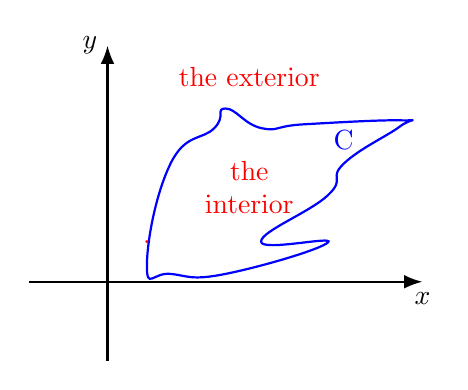
\begin{tikzpicture}[
    >=Latex, % Set default arrow tip style
    axis/.style={->, thick}, % Style for axes
    blob/.style={blue, thick}, % Style for the blob curve
    labelstyle/.style={red}, % Style for interior/exterior labels
    curvelabel/.style={blue} % Style for curve label C
]

    % Axes
    \draw[axis] (-1, 0) -- (4, 0) node[below] {$x$}; % x-axis
    \draw[axis] (0, -1) -- (0, 3) node[left] {$y$}; % y-axis

    % Draw the Blob using plot smooth cycle
    \draw[blob] plot [smooth cycle, tension=0.8] coordinates {
(0.8, 0.1)        
        (0.5, 0.2)
                (0.8, 1.5)
        (1.355, 1.95)
        (1.5, 2.2) 
        (1.96, 1.95)
        (2.5, 2.0)
        (3.73, 2.05) 
(3.71, 1.97)        
        (3.0, 1.5)
        (2.8, 1.1)
        (1.95, 0.51)
        (2.8, 0.5) 
                (1.5, 0.1) 
               % 
 %       (0.163, 0.024)
%(0.9, 0.3)
%(1.33, 0.36)
%
%(2.67, 0.7)
%(2.74, 1.19)
%(2.88, 1.28)
%(3.16, 1.48)
%(3.35, 1.92)
%()
%
%
%(4.7, 2.2)
%(4.85, 2.73)
       %# (0.07, 0.06)
       % (0.48 ,0.33)
    };
    
    \node[red, thick] at (0.5,0.5) {.};

    % Add Labels
    % Interior Label (centered inside)
    \node[labelstyle, align=center] at (1.8, 1.2) {the \\ interior};

    % Exterior Label (above the blob)
    \node[labelstyle] at (1.8, 2.6) {the exterior};

    % Curve Label C (near the curve on the right)
    \node[curvelabel] at (3.0, 1.8) {C};

\end{tikzpicture}
\end{document}